\documentclass[aspectratio=169]{beamer}
\usetheme[progressbar=none]{metropolis}           % Use metropolis theme
%\input{metropolis-settings.tex}
\usepackage[T1]{fontenc}
\usepackage[italian]{babel}
\usepackage[sfdefault]{FiraSans}
\usepackage{graphicx}
\graphicspath{{../img/}}

\title{Algoritmo di tagging di raggi cosmici\\in un sistema di acquisizione triggerless\\\mbox{per un esperimento di fisica di particelle su fascio}}
\date{Anno Accademico 2022/2023}
\author{Antonio Ghinassi}
\institute{Alma Mater Studiorum $\cdot$ Università di Bologna}

\begin{document}
  \maketitle
  \setbeamertemplate{frame footer}{\insertinstitute}%Alma Mater Studiorum $\cdot$ Università di Bologna}
  %\section{First Section}
  \begin{frame}{Raggi cosmici}
    
\begin{columns}[onlytextwidth,T]
  \begin{column}{.45\linewidth}
    testo
  \end{column}
  \begin{column}{.45\linewidth}
    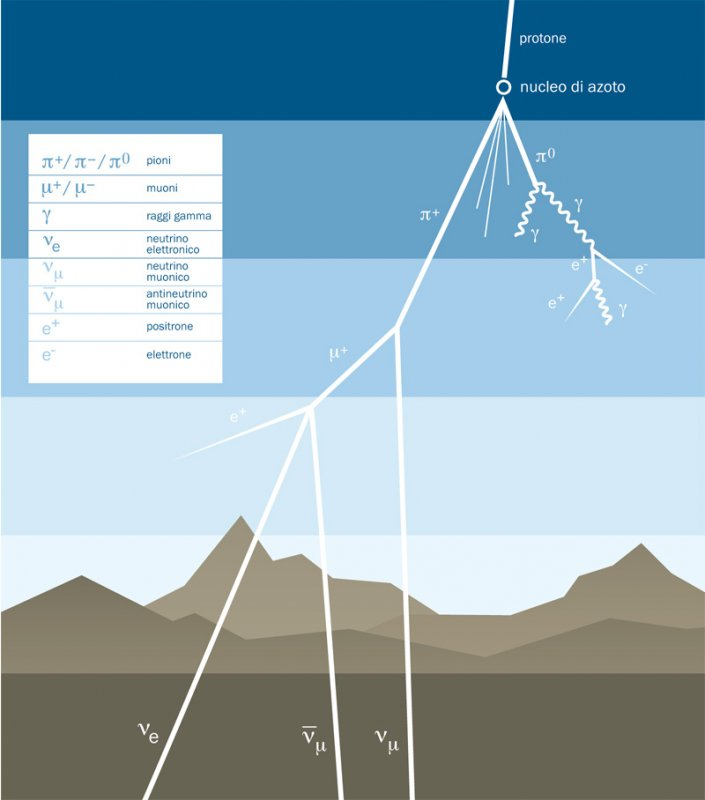
\includegraphics[scale=0.23]{cosmic.jpg}
  \end{column}
\end{columns}

  \end{frame}
  \begin{frame}{Acquisizione dati \emph{triggerless}}
    Hello, world!
  \end{frame}
  \begin{frame}{TriDAS}
    Hello, world!
  \end{frame}
  \begin{frame}{TriDAS @ JLab}
    Hello, world!
  \end{frame}
  \begin{frame}{Algoritmo \texttt{I}}
    Hello, world!
  \end{frame}
  \begin{frame}{Algoritmo \texttt{II}}
    Hello, world!
  \end{frame}
  \begin{frame}{Algoritmo \texttt{III}}
    Hello, world!
  \end{frame}
  \begin{frame}{Strumenti di analisi e test}
    Hello, world!
  \end{frame}
  \begin{frame}{Conclusioni}
    Hello, world!
  \end{frame}
  \begin{frame}[standout]
      Grazie per l'attenzione.
  \end{frame}
\end{document}
